\documentclass[serif,mathserif,final]{beamer}
\mode<presentation>{\usetheme{Lankton}}
\usepackage{amsmath,amsfonts,amssymb,pxfonts,eulervm,xspace}
\usepackage{graphicx}
\usepackage{mathrsfs}
\usepackage{subfigure}
\graphicspath{{./figures/}}
\usepackage[orientation=landscape,size=custom,width=121.92,height=91.44,scale=1.3,debug]{beamerposter}

%-- Header and footer information ----------------------------------
\newcommand{\footleft}{}
\newcommand{\footright}{}
\title{Epidemiological Methods for Examining Bullying}
\author{Andrea Bruder and Kaitlyn Martinez}
\institute{Department of Mathematics and Computer Science, Colorado College, Colorado Springs, CO}
%-------------------------------------------------------------------


%-- Main Document --------------------------------------------------
\begin{document}
\begin{frame}{}
  \begin{columns}[t]

    %-- Column 1 ---------------------------------------------------
    \begin{column}{0.23\linewidth}

      %-- Block 1-1 ABSTRACT
      \begin{block}{Abstract} \small
Bullying is defined as a specific type of aggression, in which the behavior is intended to harm or disturb, the behavior occurs repeatedly, and there is an imbalance of power $[5]$. The results are significant psychological damage in the victim, but also in the bully. Studies report the number of bullied children in middle schools as between 4\% and 82\% $[2]$. The goals of our study are to understand how bullying behavior spreads in a population of adolescents, and to examine the impacts of the most common bullying intervention strategies. We propose a mathematical model, in which we subdivide a population of adolescents into those susceptible to being bullied, victims of bullying, those who turn into bullies after being bullied, those who do not engage in bullying behavior after being bullied, and a recovered group. The model is parameterized using data on the prevalence of bullying. An analysis of the model shows that whether the bullying behavior spreads in a population depends on the rate at which susceptible individuals are bullied, the probability of bullied individuals turning into bullies themselves, and on the duration of the bullying in each instant. Numerical simulations of the model including the most common intervention strategies suggest that the Traditional Disciplinary Approach, although commonly implemented, is the least effective of the intervention strategies we studied. 
\end{block}

      %-- Block 1-2 INTRO
      \begin{block}{Statistical Data on Bullying}
       \begin{itemize}
\small\item $30\%$ of all children are involved in bullying behaviors, either as a bully, victim, or both $[2]$. 

\item In small specific studies it was found that the number of bullied children could be as low as $4\%$ to as high as $82\%$. In larger sampling populations, the percentage of children bullied is between $12\%$ and $25\%$ $[2][4]$. 
%%citations!! 

\item The percentage of children who are bullies is between $8\%$ and $13\%$ $[2][5]$.
%%citations!!

\item Bullying is linked to many adverse effects like poor academic performance, impaired social skills, and more alarmingly also increases rates of suicide and school shootings. 

\end{itemize}
      \end{block}

      %-- Block 1-3 METHODS
      \begin{block}{Methods in Epidemiology} \small
       Compartmental models are widely used in epidemiology to study the spread of infectious diseases $[3]$. While these methods have been applied to social issues such as alcohol and drug use $[8]$ or crime $[7]$, to our knowledge, they have not been used to study the phenomenon of bullying.

In epidemiology, a population of individuals is compartmentalized into the subpopulations of susceptible, infected, and recovered individuals. Individuals may move between the compartments according to the model assumptions as shown in Figure \ref{fig:SIR}. 

\begin{figure}[H]
\centering
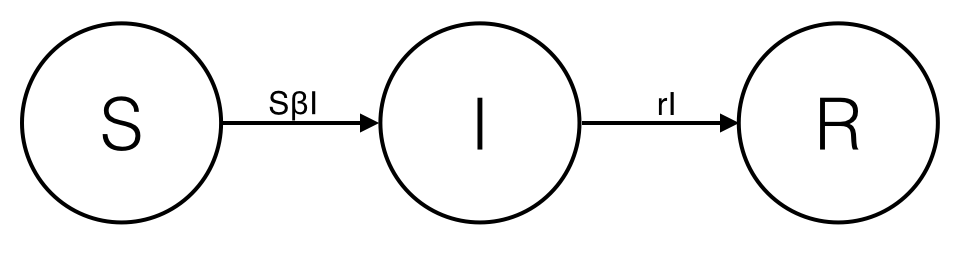
\includegraphics[width=.65\textwidth]{SIR}
\vspace{-10pt}
\caption{\label{fig:SIR} SIR Model for infectious diseases}
\end{figure}
Bullying spreads in a population much like an infectious disease, that is, a susceptible individual who encounters a bully may be exposed to bullying. (Compare to a susceptible individual who encounters an infectious individual and is exposed to the infectious disease.) We approach bullying from an epidemiological point of view and use statistical data about the prevalence of bullying to parameterize our model.

In the study of infectious diseases, the basic reproductive number, $\mathscr{R}_0$, determines how many secondary infections are generated on average from introducing one infectious individual into a susceptible population [3]. If $\mathscr{R}_0>1$, then the disease spreads resulting in an epidemic, and if $\mathscr{R}_0<1$, the disease does not spread. In the context of bullying, we interpret the basic reproductive number as the average number of individuals exposed to bullying if one bully is introduces into a population of susceptible individuals. 
      \end{block}

    \end{column}%1

    %-- Column 2 ---------------------------------------------------
    \begin{column}{0.40\linewidth}

      %-- Block 2-1 BASIC MODEL
      \begin{block}{The Mathematical Model}
       \textbf{Model Assumptions} \small
\begin{itemize}
\item Bullying spreads much like an infectious disease, passing the dynamic on through an interaction between in “infected” individual (the bully) and a “susceptible” individual (the victim).
\item Only bullies are “infectious”. Bullying spreads via interactions between bullies and susceptible individuals. 
\item After being exposed to bullying, a victim can either become a bully themselves or become a non-bully. We disregard those who are both bullies and are bullied themselves.
\item An individual can spontaneously turn into a bully with a low probability $c$. 
\item After being exposed to bullying, a victim can either become a bully themselves or become a non-bully. 
\item Both bullies and non bullies can recover.
\item “Immunity” does not last. A proportion d of the recovered population are reintroduced into the susceptible population.
\end{itemize}
\begin{minipage}{.68\textwidth}
\begin{figure}[H]
\centering
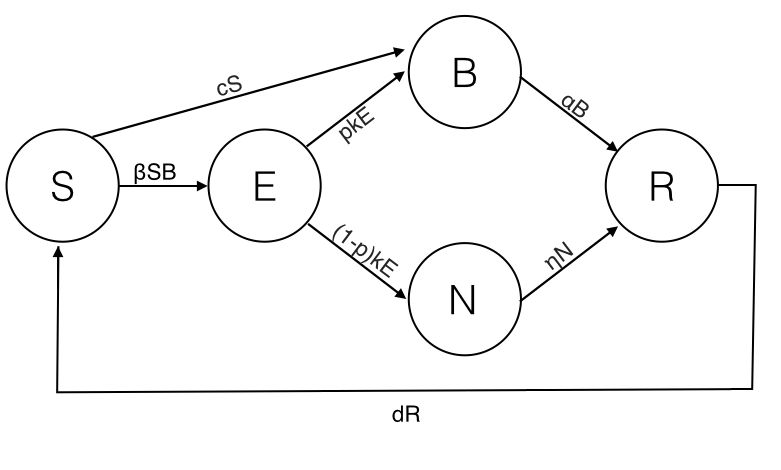
\includegraphics[width=0.9\linewidth]{Compartmental_Model}
\vspace{-40pt}
\caption{\label{fig:Compartmental_Model}
The SEBNR Bullying Model. Susceptible individuals ($S$), exposed individuals ($E$), non-bullies ($N$), bullies ($B$), and recovered individuals ($R$) move between model compartments according to the model assumptions.}
\end{figure}
\end{minipage}
\begin{minipage}{.3\textwidth}
$S(t)$: Number of susceptible\\ \hphantom{aaaa} individuals at time $t$\\
$E(t)$: Number of individuals \\\hphantom{aaaa} exposed to bullying at time $t$\\
$B(t)$: Number of bullies at time $t$\\
$N(t)$: Number of non-bullies \\\hphantom{aaaa} at time $t$\\
$R(t)$: Number of recovered\\ \hphantom{aaaa} individuals at time $t$
\end{minipage}
\begin{minipage}{.29\textwidth}
\normalsize
\begin{equation*}\label{eq:basic+}
\begin{aligned}
%P(t)&=S+E+B+N+R\\
S'(t)&=-\beta B S+dR -cS\\
E'(t)&=\beta B S -k E\\
B'(t)&=p k E +cS -\alpha B\\
N'(t)&=(1-p) k E - \eta N\\
R'(t)&=\eta N +\alpha B-dR,\\
\end{aligned}
\end{equation*}
\end{minipage}
\begin{minipage}{.69\textwidth}
\begin{table}[H]
\label{table:parameterssimple}
\begin{tabular}{cl}
\hline
 Parameter & Meaning \\ \hline 
 \small $\beta$ & \small rate of infection \\ 
$c$ &  proportion of susceptible population that spontaneously become bullies \\ 
$p$ & \small probability of becoming a bully after being bullied  \\ 
$k$ & $\small \frac{1}{k}$ is the amount of time spent exposed to bullying \\ 
$\eta$ & $\small \frac{1}{\eta}$ is the amount of time spent as a non-bully \\
$\alpha$ & $\frac{1}{\alpha}$ is the amount of time spent as a bully \\ 
$d$ &   proportion of children that lose their immunity to bullying 
\end{tabular}
\end{table}
\end{minipage}

      \end{block}

      %-- Block 2-2 RESULTS
      \begin{block}{Results}
      \vspace{-20pt}
      \begin{figure}[H]
\centering
\begin{subfigure}[Example of a system with $R_0<1$. $R_0=0.7645$ when the initial population is $100$ and the parameter values are $\alpha=.99$, $\beta=.087$, $p=.087$, $c=0$, $k=.95$, $\eta=.6$, and $d=.1$. This results in a disease free equilibrium.]{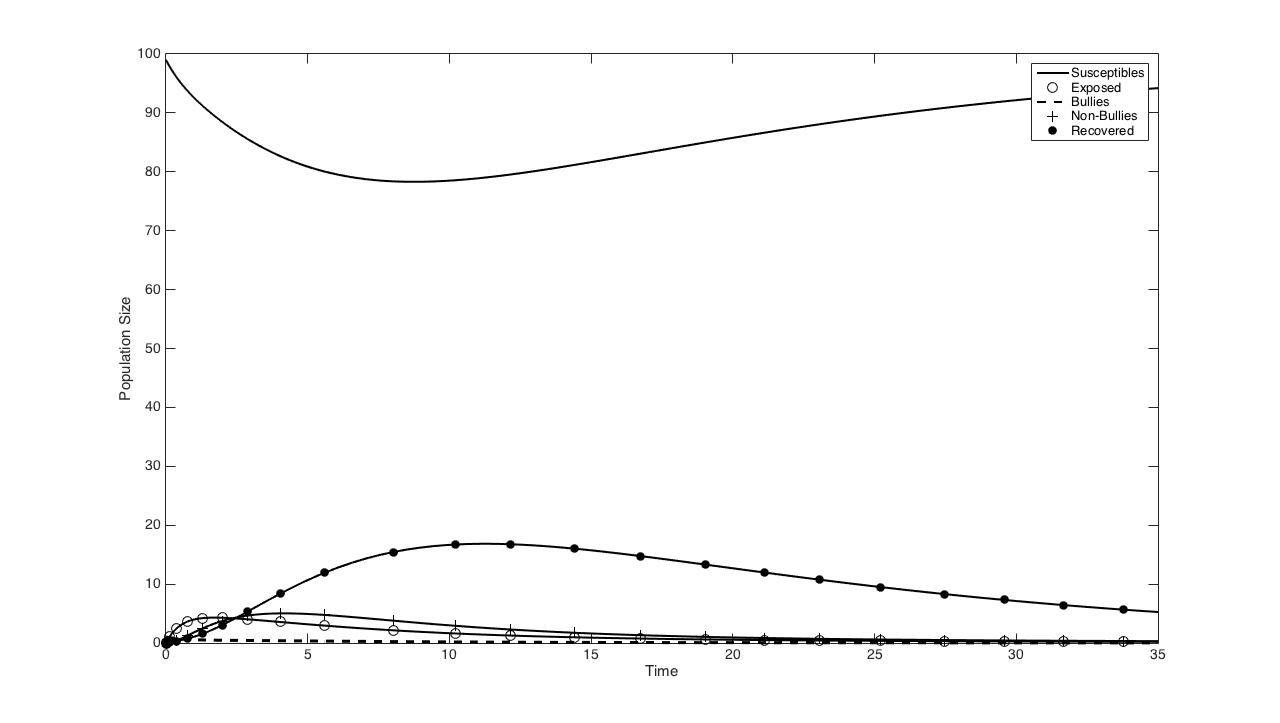
\includegraphics[width=.47\textwidth]{R0lt1}}
\end{subfigure}
~
\begin{subfigure}[Example of a system with $R_0>1$. $R_0=6.667$ when the initial population is $100$ and the parameter values are $\alpha=.75$, $\beta=.25$, $p=.2$, $c=0$, $k=.95$, $\eta=.6$, and $d=.1$. This results in an endemic equilibrium.]{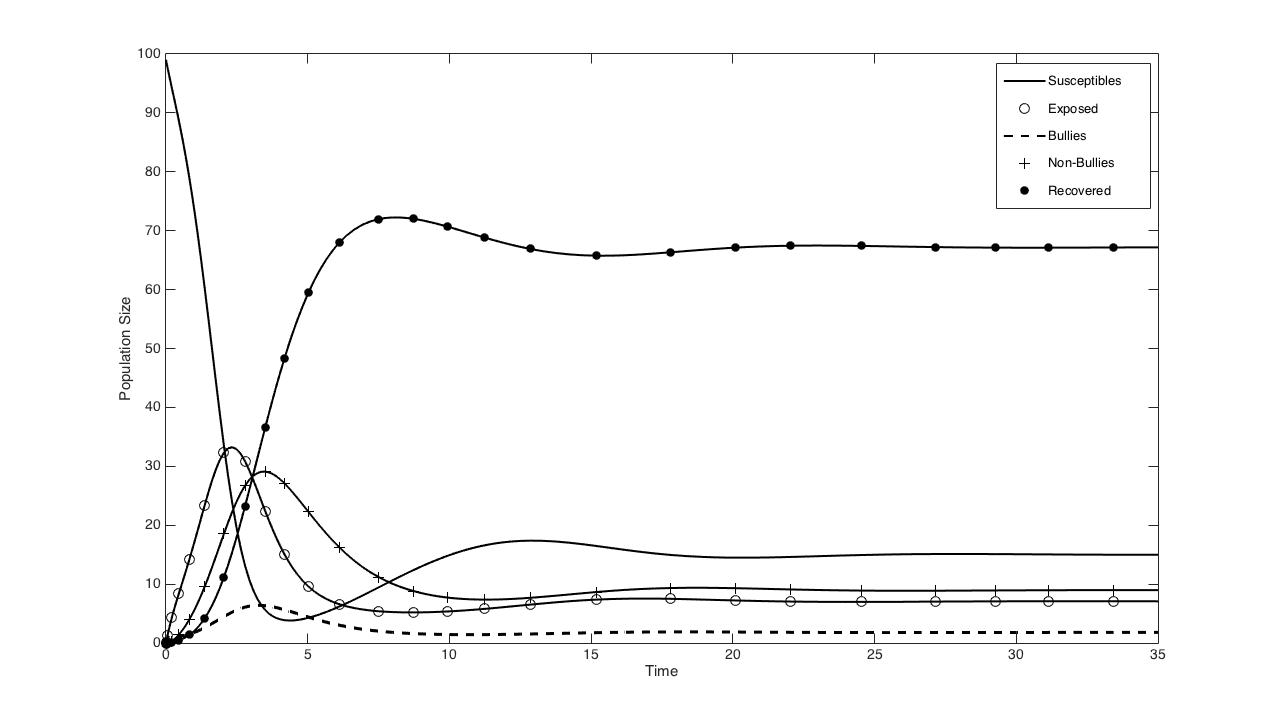
\includegraphics[width=.47\textwidth]{R0gt1}}\end{subfigure}\caption{\label{fig:R0} Systems at different equilibrium states depending on the value of $R_0$. }
\end{figure}
      \end{block}

      %-- Block 2-3
%       \begin{block}{Pictures}
%         %\begin{figure}[htb]
%          % \centering
%           %\includegraphics[width=.6\columnwidth]{science}
%         %\end{figure}
%       \end{block}

    \end{column}%2

    %-- Column 3 ---------------------------------------------------
    \begin{column}{0.35\linewidth}

      %-- Block 3-1 Intervention Model
      \begin{block}{Intervention Model} \small
%          \begin{figure}[htb]
%          \centering
%           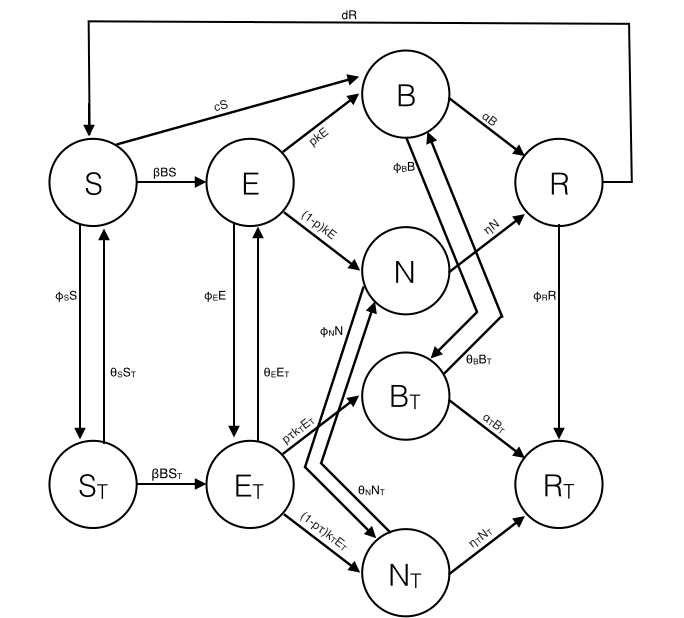
\includegraphics[width=.6\columnwidth]{Compartmental_TreatmentModel}\caption{\label{fig:Compartmental_TreatmentModel}
% The general model incorporating intervention strategies that models the interactions of individuals that have not experienced intervention and those that have. This model can be tailored to match specific strategies used in schools today.}
%         \end{figure}
        
    \begin{figure}[H]
\centering
\begin{subfigure}[The Compartmental Model for the Traditional Disciplinary Approach. In this Approach, a proportion of the bullies is disciplined and moves into a "treated" compartment. The intervention may fail at a certain rate, in which case the treated individuals move back into the Bully compartment.]{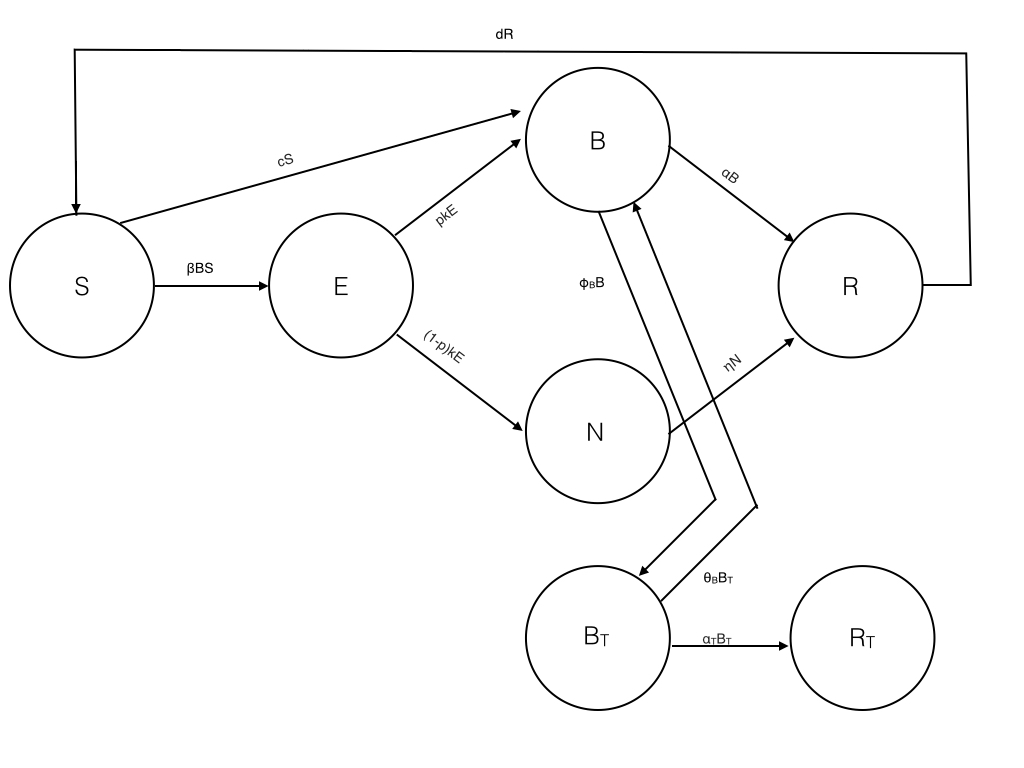
\includegraphics[height=.355\textwidth]{Intervention_TACompartments}}\end{subfigure}
~
\begin{subfigure}[The Strengthening the Victim Approach. A proportion of the susceptible and exposed individuals are moved into "treated" compartments. The intervention may fail, and "treated" individuals may move back to their original compartments.]{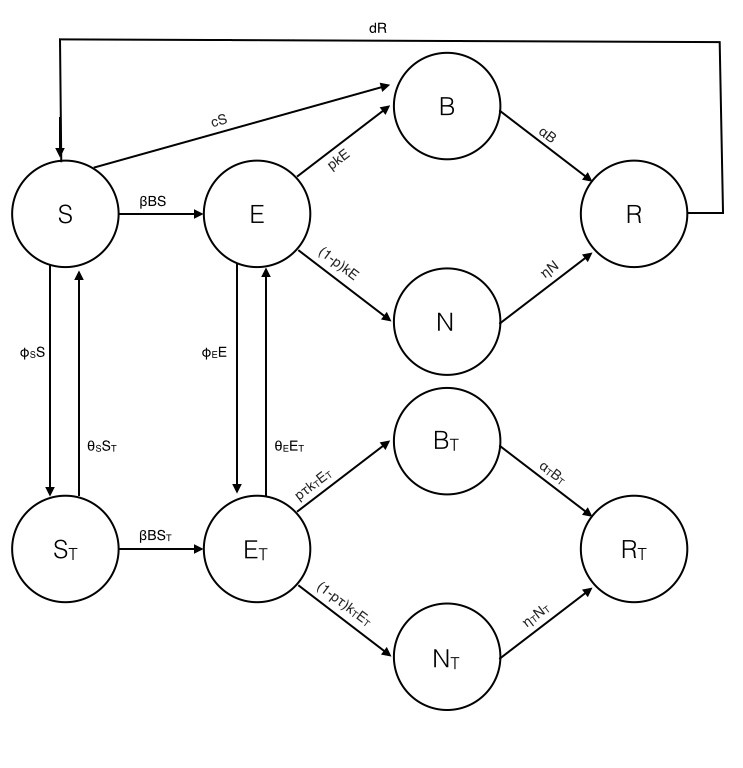
\includegraphics[height=.355\textwidth]{Intervention_SVCompartments}}
\end{subfigure}
% \caption{\label{fig:R0} for $S_0=50$ - Parameter Values: (a) $R_0=.8889<1$ - $\alpha=.9$, $\beta=.16$, $p=.1$, $c=0$, $k=.95$, $\eta=.6$, and $d=.1$. (b) $R_0=2.222>1$ - $\alpha=.9$, $\beta=.4$, $p=.1$, $c=0$, $k=.95$, $\eta=.6$, and $d=.1$.}
\end{figure}     
%         \begin{figure}[H]
% \centering
% \subfigure[]{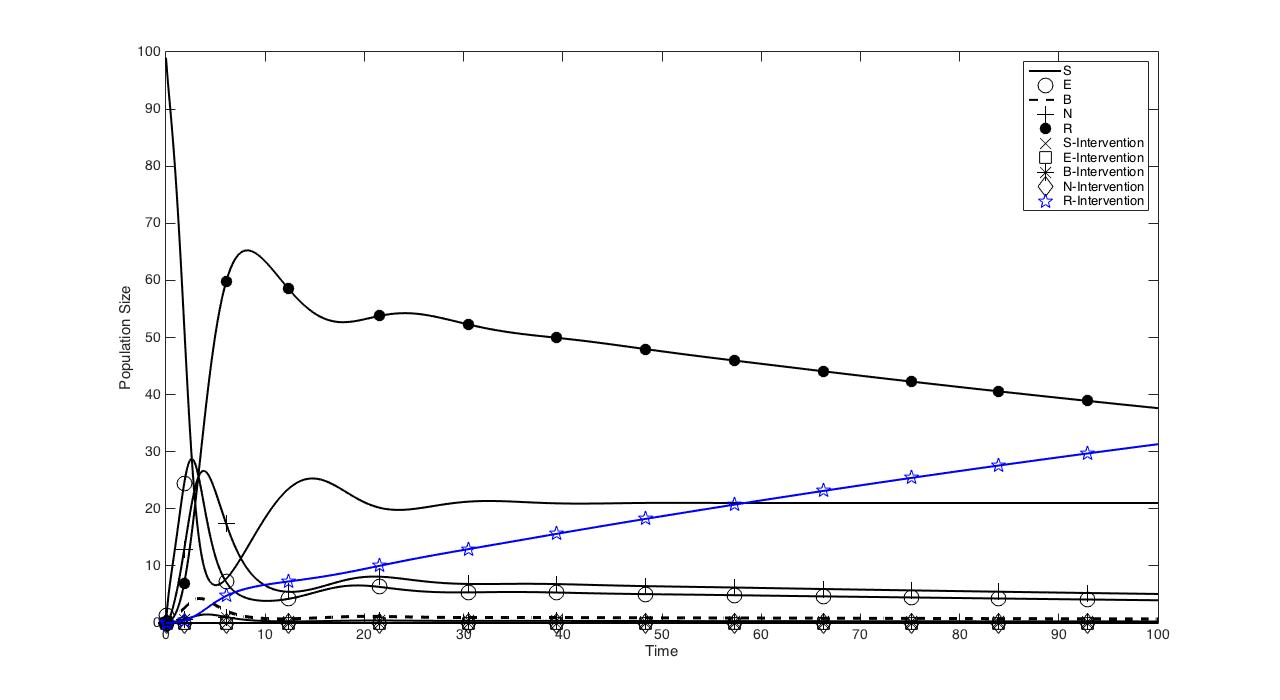
\includegraphics[width=.475\textwidth]{Present_TraditionalApproach}}\qquad
% \subfigure[]{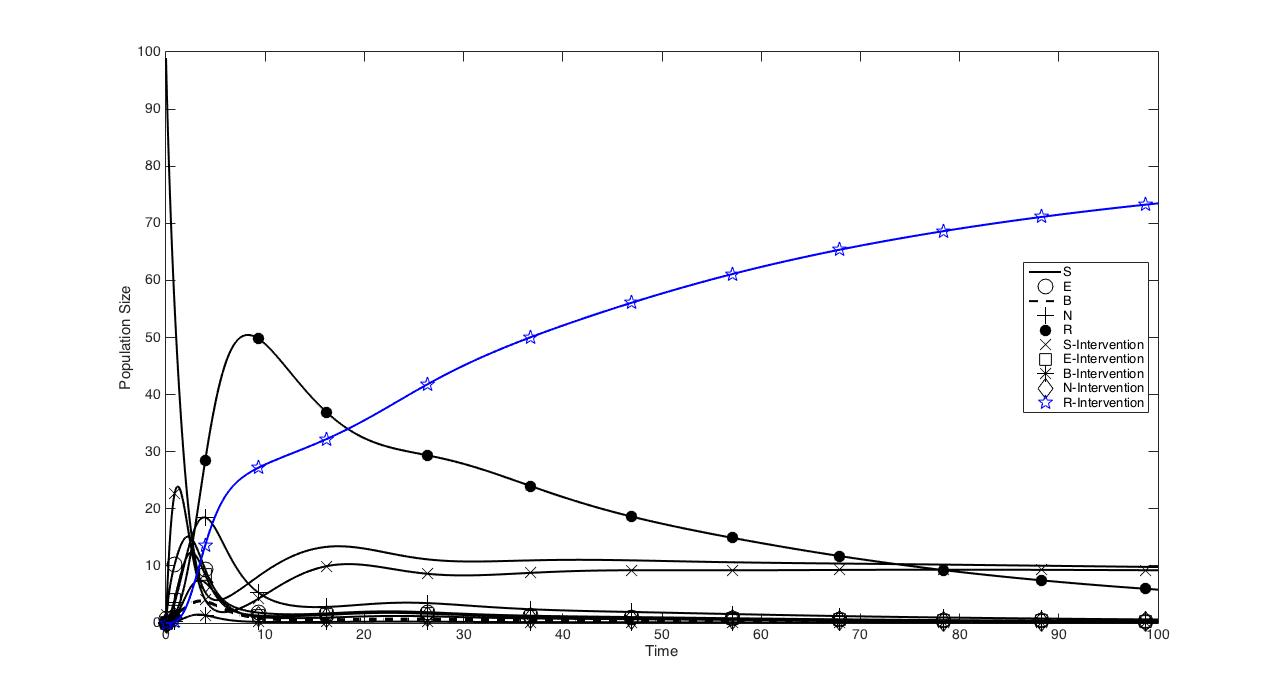
\includegraphics[width=.475\textwidth]{Present_StrengthVic_SE}}
% %\caption{\label{fig:R0} for $S_0=50$ - Parameter Values: (a) $R_0=.8889<1$ - $\alpha=.9$, $\beta=.16$, $p=.1$, $c=0$, $k=.95$, $\eta=.6$, and $d=.1$. (b) $R_0=2.222>1$ - $\alpha=.9$, $\beta=.4$, $p=.1$, $c=0$, $k=.95$, $\eta=.6$, and $d=.1$.}
% \end{figure}
\begin{figure}[H]
\centering
\begin{subfigure}[Numerical simulation of an implementation of the Traditional Disciplinary Approach that assumes that $50\%$ of bullies undergo intervention and that $50\%$ of those interventions fail. After one-hundred days the population is only $30\%$ recovered.]{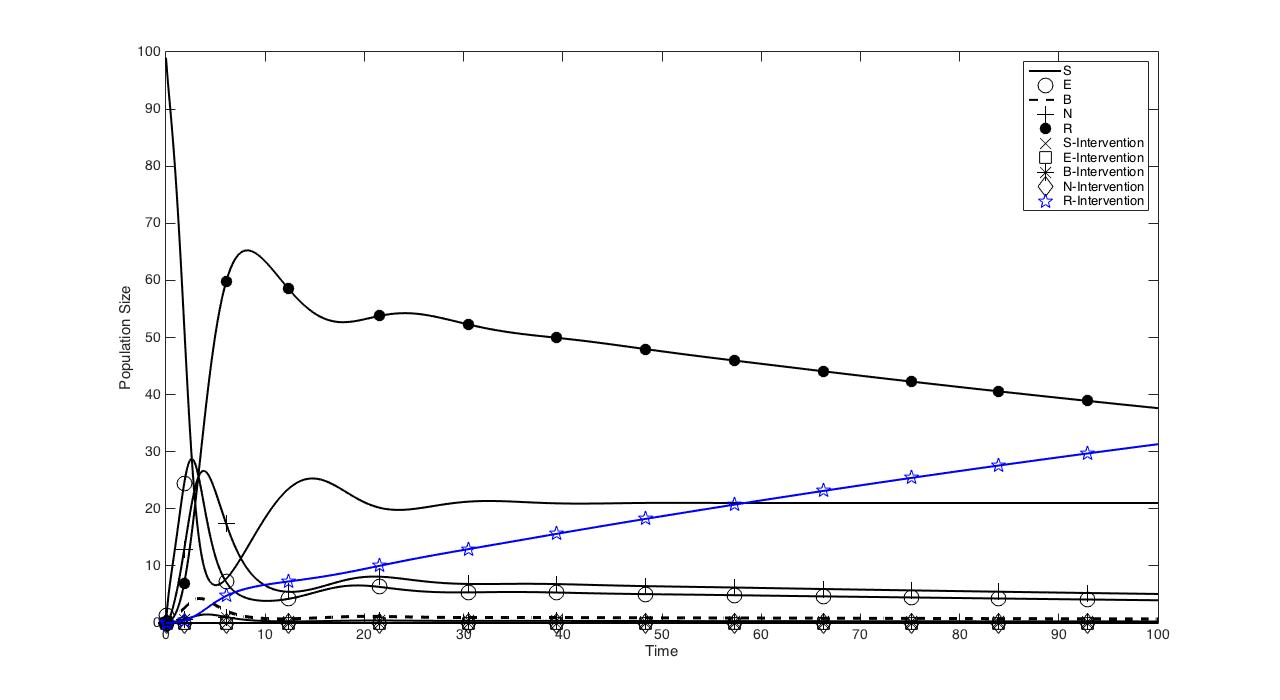
\includegraphics[width=.47\textwidth]{Present_TraditionalApproach}}
\end{subfigure}
~
\begin{subfigure}[Numerical simulation of an implementation of the Strengthening the Victim that assumes that $50\%$ of susceptible and exposed individuals undergo intervention and that $50\%$ of those interventions fail. After fifty days the population is $70\%$ recovered.]{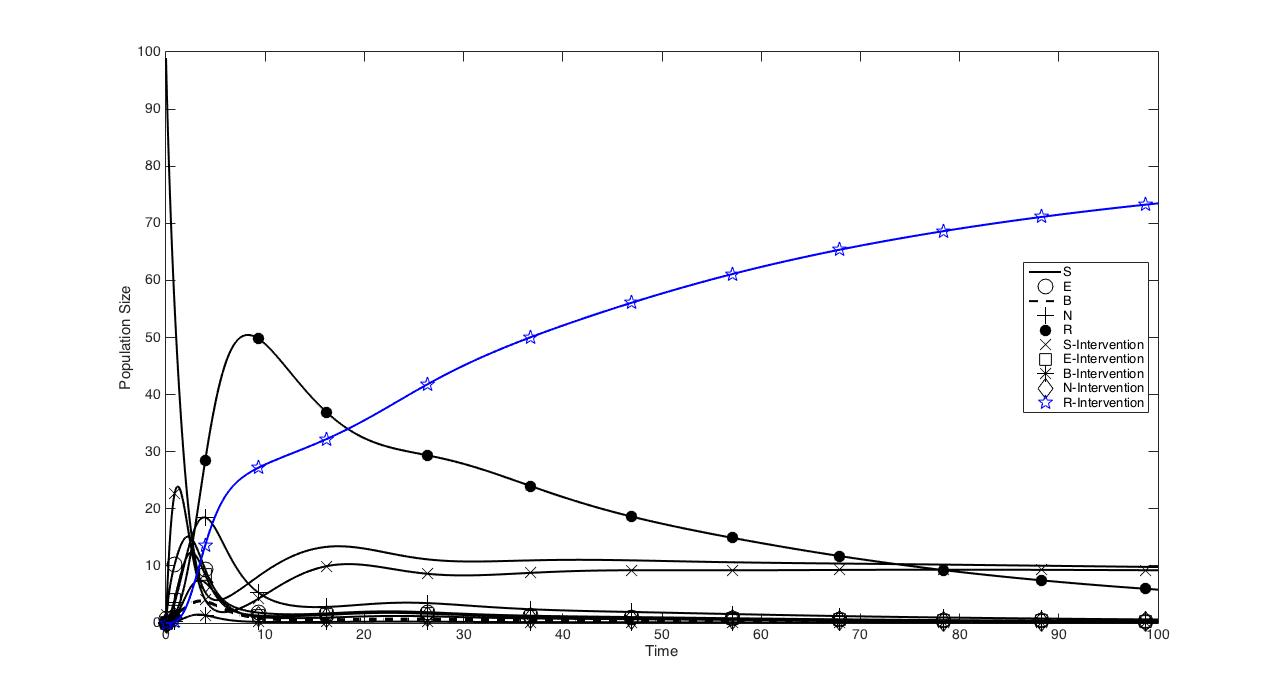
\includegraphics[width=.47\textwidth]{Present_StrengthVic_SE}}\end{subfigure}
\end{figure}
The Traditional Approach is by far the most common intervention strategy, yet by our numerical simulations, it is the least effective both in terms of the long and short term behavior of the system. Rampant bullying occurs at the introduction of a small number of bullies, and it takes a long time for the population to recover. In contrast, the Strengthening the Victim Approach has better long term outcomes than that of the Traditional Approach. 
 Under our assumptions about effectiveness of each intervention strategy, the Strengthening the Victim Approach boasts significantly faster recovery than that of the Traditional Approach. The Strengthening the Victim approach does still have frequent bullying that occurs after the introduction of bullies into the system, however the impact is lower and the system recovers faster. 
      \end{block}

      %-- Block 3-2 Conclusions/Discussion
      \begin{block}{Conclusions} \small
Whether the bullying behavior spreads in a population depends on the rate at which susceptible individuals are bullied, the probability of bullied individuals turning into bullies themselves, and on the duration of the bullying in each instant. Numerical simulations of the model including the most common intervention strategies suggest that the Traditional Disciplinary Approach, although commonly implemented, is the least effective of the intervention strategies we studied.
      \end{block}

      %-- Block 3-3 References
      \begin{block}{References} \tiny
        $[1]$ J. Arino et al.: Simple models for containment of a pandemic. Journal of The Royal Society Interface , $3(8):453-457$, June 22 2006.\\
 $[2]$ K. Stassen Berger: Update on bullying at school: Science forgotten? Developmental Review , $27(1): 90-126$, 3 2007.\\
 $[3]$ F. Brauer and C. Castillo-Ch ́avez. Mathematical Models in Population Biology and Epidemiology. Texts in applied mathematics. Springer, 2001.\\
 $[4]$ W. Craig et al: A cross-national profile of bullying and victimization among adolescents in 40 countries. International Journal of Public Health, 54(2):216–224, 2009.\\
 $[5]$ T. Nansel: Bullying behaviors among US youth: Prevalence and association with psychosocial adjustment. JAMA, $285(16):2094-2100$, April 25 2001.\\
 $[6]$ K. Rigby. Bullying Interventions in Schools: Six Basic Approaches . Wiley, 2012. 2012020896.\\
 $[7]$ M. Short et al.: Dissipation and displacement of hotspots in reaction-diffusion models of crime. Proceedings of the National Academy of Sciences, 107(9):3961–3965, 2010.\\
 $[8]$ Emma White and Catherine Comiskey. Heroin epidemics, treatment and ODE modelling. Mathe- matical Biosciences, 208(1):312 – 324, 2007.

      \end{block}
%-- Block 3-4 Acknowledgements
\begin{block}{Acknowledgements} \small
        This research was supported by a 2014 Faculty-Student Collaborative Research Grant from Colorado College.
      \end{block}
    \end{column}%3

  \end{columns}
\end{frame}
\end{document}

